\documentclass[conference]{IEEEtran}
\IEEEoverridecommandlockouts
\usepackage{cite}
\usepackage{amsmath,amssymb,amsfonts}
\usepackage{graphicx}
\usepackage{booktabs}
\usepackage{tabularx}
\usepackage{textcomp}
\usepackage{xcolor}
\usepackage{url}
\usepackage{microtype}

% Evita estouros de margem em colunas estreitas e melhora o espaçamento de floats
\setlength{\emergencystretch}{1.5em}
\setlength{\textfloatsep}{10pt plus 2pt minus 2pt}
\setlength{\floatsep}{8pt plus 2pt minus 2pt}
\setlength{\intextsep}{8pt plus 2pt minus 2pt}

\def\BibTeX{{\rm B\kern-.05em{\sc i\kern-.025em b}\kern-.08em
T\kern-.1667em\lower.7ex\hbox{E}\kern-.125emX}}

\begin{document}

\title{Polymorphic SRAM Using 2D Transistors for Enhanced Hardware Security}

\author{\IEEEauthorblockN{Bernardo Vale}
\IEEEauthorblockA{\textit{UFMG}}
\and
\IEEEauthorblockN{Danilio Costa}
\IEEEauthorblockA{\textit{UFMG}}
\and
\IEEEauthorblockN{Felipe Melo}
\IEEEauthorblockA{\textit{UFMG}}
\and
\IEEEauthorblockN{Gabriel Ferreira}
\IEEEauthorblockA{\textit{UFMG}}
}

\maketitle

\begin{abstract}
Static random-access memory (SRAM) arrays store sensitive cryptographic keys, firmware, and runtime states in modern integrated circuits, making them primary targets for physical probing, data-remanence extraction, and unauthorized tampering. Conventional silicon CMOS SRAM cells rely on fixed chemical doping, preventing transistor-level functional reconfiguration without adding peripheral area and latency overheads. This paper presents the design, behavioral modeling, and circuit-level security evaluation of a polymorphic six-transistor (6T) SRAM cell based on two-dimensional (2D) ambipolar black phosphorus Schottky-barrier field-effect transistors (BP SB-FETs) in a fully open-source \texttt{ngspice-47} and Python flow. By translating 4D experimental lookup tables with bilateral source referencing and gate-specific saturation curves, our native SPICE subcircuit achieves $R^2 \ge 0.99977$ against Synopsys HSPICE and reduces \textit{p-FET} output error by $196\times$ at $V_{g2}=-1.5\ \text{V}$. Exploiting runtime electrostatic polarity gating under strictly fixed power rails ($V_{DD}=1.0\ \text{V}$, $V_{SS}=0.0\ \text{V}$), the 6T SRAM cell operates as a standard bistable memory under the authorized key ($\text{Key}=0$, $\Delta V_{\mathrm{Key0}}=0.9747\ \text{V}$, $\mathrm{SNM}_{\mathrm{Hold}}=167.12\ \text{mV}$), whereas asserting an unauthorized key ($\text{Key}=1$) dynamically inverts pull-up and pull-down polarities, converting the cross-coupled inverters into monostable source followers that instantaneously erase stored data ($\mathrm{SNM}=0.00\ \text{mV}$, $\Delta V_{\mathrm{Collapse1}}=0.0841\ \text{V}$) and block subsequent write attempts. Furthermore, we diagnose destructive \textit{Read Disturb} during unassisted reads and resolve it via \textit{Wordline Underdrive Read-Assist} ($\mathrm{WL}=0.30\ \text{V}$), restoring $\mathrm{SNM}_{\mathrm{Read,Assist}}=66.23\ \text{mV}$ with zero additional transistors.
\end{abstract}

\begin{IEEEkeywords}
Polymorphic SRAM, 2D Transistors, Reconfigurable FETs, Black Phosphorus, Hardware Security, Static Noise Margin.
\end{IEEEkeywords}

\section{Introduction}
Field-effect transistors (FETs) are the fundamental active building blocks of modern digital integrated circuits (ICs), where billions of complementary \textit{p-type} (\textit{p-FET}) and \textit{n-type} (\textit{n-FET}) devices form combinational logic and embedded memory arrays \cite{sze2007, rabaey2003, moore1998}. In conventional silicon CMOS technology, transistor conduction polarities are permanently established during manufacturing via substitutional chemical doping, rendering each device's electrical role static post-fabrication \cite{sze2007, wu2021}. Meanwhile, the globalization of the semiconductor supply chain has exposed integrated systems to severe hardware security threats, including intellectual property (IP) piracy, reverse engineering via high-resolution imaging, physical microprobing, and cold-boot or data-remanence attacks targeting volatile on-chip memories \cite{rostami2014, shamsi2019, quadir2016, halderman2009lest}.

Embedded static random-access memory (SRAM) is particularly critical from a security standpoint because it holds cryptographic keys, device identifiers, and intermediate plaintexts during execution, leaving systems vulnerable to cold-boot extraction, data-remanence probing, and hardware Trojan tampering \cite{halderman2009lest, bhunia2014hardware}. Conventional CMOS memory protection mechanisms---such as peripheral encryption wrappers, dummy-contact layout camouflaging, and power-gating zeroization circuits---introduce substantial silicon area, power, and access-latency penalties \cite{vijayakumar2016, xie2017, yasin2016, kamali2020}. Moreover, zeroization schemes that rely on disconnecting or swapping power supply rails can be bypassed by adversaries clamping external supply pins or detected via power-rail monitoring.

Reconfigurable field-effect transistors (RFETs), or polymorphic transistors, overcome the rigidity of static doping at the device physics level \cite{heinzig2012, wu2021, mikolajick2017, mikolajick2021}. Utilizing undoped low-dimensional channels with electrostatic polarity gating, a single RFET can dynamically switch between \textit{p-FET} and \textit{n-FET} conduction modes during runtime \cite{nakaharai2015, demarchi2012, rhee2025}. While prior polymorphic circuit studies have largely focused on combinational logic gates (such as \texttt{NAND}/\texttt{NOR} and \texttt{XOR}/\texttt{XNOR} cells) \cite{resta2018, benjamaa2011, galderisi2022, bi2016}, applying runtime polarity inversion to sequential storage elements enables native, zero-overhead memory protection \cite{wu2021}.

In this paper, we investigate a polymorphic six-transistor (6T) SRAM cell implemented with two-dimensional (2D) black phosphorus Schottky-barrier FETs (BP SB-FETs) for enhanced hardware security. Rather than permuting supply rails, the architecture employs polarity-controlled retention locking (\textit{Mechanism B}), keeping $V_{DD}$ and $V_{SS}$ strictly fixed while using a runtime cryptographic key to invert the conduction polarities of the cross-coupled inverters. Under the authorized key ($\text{Key}=0$), the cell exhibits robust bistable retention; under an unauthorized key ($\text{Key}=1$), simultaneous inversion of pull-up and pull-down devices collapses bistability into a monostable state, instantaneously zeroizing stored data and preventing unauthorized overwrites.\footnote{The open-source \texttt{ngspice-47}/Python codebase developed in this project---including supplementary experiments on ultra-low-voltage inverters, polymorphic combinational gates, differential power analysis (DPA) Pareto benchmarks, non-nominal voltage boundaries, and an interactive web simulator---is available at \url{https://github.com/BernardooVale/tp_nano}.}

To enable accurate and reproducible circuit-level verification without proprietary commercial simulators, we make the following core contributions:
\begin{enumerate}
    \item \textbf{Open-Source 4D BP SB-FET Modeling:} We translate 4D experimental BP SB-FET lookup tables into a native \texttt{ngspice-47} behavioral subcircuit (\texttt{bp\_ari\_\allowbreak ngspice.lib} \texttt{v2}) featuring bilateral source referencing for bidirectional SRAM pass-gates and full capture of the $V_{g2}=-1.5\ \text{V}$ flat-band shift ($\Delta V_{fb} \approx -0.25\ \text{V}$), achieving $R^2 \ge 0.99977$ against Synopsys HSPICE.
    \item \textbf{Polarity-Controlled 6T SRAM Retention Locking:} We validate fixed-rail retention locking across a four-phase $30\ \text{ns}$ transient protocol, demonstrating stable retention under $\text{Key}=0$ ($\Delta V_{\mathrm{Key0}}=0.9747\ \text{V}$) and immediate state collapse under $\text{Key}=1$ ($\Delta V_{\mathrm{Collapse1}}=0.0841\ \text{V}$).
    \item \textbf{Flat-Band Symmetry \& Read-Assist Optimization:} Through butterfly-curve Static Noise Margin (SNM) extraction, we show that tuning $V_{g2,\mathrm{PU}}$ from $-0.5\ \text{V}$ to $-0.2\ \text{V}$ recovers $\mathrm{SNM}_{\mathrm{Hold}}$ from $49.4\ \text{mV}$ to $167.12\ \text{mV}$ without device resizing, and we mitigate destructive \textit{Read Disturb} via \textit{Wordline Underdrive Read-Assist} ($\mathrm{WL}=0.30\ \text{V}$, $\mathrm{SNM}_{\mathrm{Read,Assist}}=66.23\ \text{mV}$).
\end{enumerate}

The remainder of this paper is organized as follows. Section~II reviews the physical background of ambipolar SB-FETs and 6T SRAM stability. Section~III surveys related work on reconfigurable devices and polymorphic security primitives. Section~IV details the 4D SPICE modeling and 6T SRAM simulation methodology. Section~V presents the validation, transient, and static SNM results, and Section~VI concludes the paper.

\section{Theoretical Background}
\subsection{From Doped MOSFETs to Ambipolar SB-FETs}
To understand how a 6T SRAM cell can dynamically erase its state via gate biasing, it is necessary to contrast conventional doped transistors with undoped ambipolar nanoscale devices \cite{sze2007, wu2021}:
\begin{itemize}
    \item \textbf{Conventional Doped FETs:} In silicon MOSFETs, substitutional chemical doping fixes carrier polarity permanently during fabrication: \textit{p-FETs} conduct holes under negative gate bias to form pull-up networks tied to $V_{DD}$, whereas \textit{n-FETs} conduct electrons under positive gate bias to form pull-down networks tied to ground \cite{sze2007, rabaey2003}.
    \item \textbf{Schottky-Barrier FET (SB-FET):} Low-dimensional semiconductors such as 2D layered crystals typically avoid substitutional doping and rely on carrier injection across metal--semiconductor Schottky barriers at the source and drain interfaces \cite{svensson2011, derycke2002, schwarz2023}. Because the channel is intrinsic, SB-FETs are inherently ambipolar, permitting both electron and hole transport depending on terminal potentials \cite{martel2001, wu2021}.
    \item \textbf{Electrostatic Polarity Gating:} To enforce unipolar behavior on demand, reconfigurable SB-FETs incorporate an auxiliary polarity gate (PG, denoted $g_2$) alongside the primary control gate (CG, denoted $g$) \cite{heinzig2012, demarchi2012, nakaharai2015}. While the CG modulates the central channel barrier to switch current on and off, the polarity gate voltage ($V_{g2}$) electrostatically bends the energy bands near the contacts to thin the Schottky barrier for the desired carrier and suppress the opposite branch---configuring the transistor dynamically as an \textit{n-FET} ($V_{g2,s} > 0$) or a \textit{p-FET} ($V_{g2,s} \le 0$) \cite{sun2021, wu2021}.
\end{itemize}

\subsection{6T SRAM Bistability, SNM, and Polarity Collapse}
A standard 6T SRAM cell comprises two cross-coupled inverters (pull-up transistors \texttt{XPU1}, \texttt{XPU2} and pull-down transistors \texttt{XPD1}, \texttt{XPD2}) storing complementary voltages at nodes $q$ and $qb$, accessed via two pass-gate transistors (\texttt{XPG1}, \texttt{XPG2}) controlled by the wordline ($\mathrm{WL}$) and bitlines ($\mathrm{BL}, \mathrm{BLB}$) \cite{rabaey2003}. Data retention requires regenerative loop gain ($|A_v| > 1$), quantified statically by the Static Noise Margin (SNM)---the side length of the largest square inscribable within the lobes of the cross-coupled voltage transfer characteristics (butterfly curve) \cite{seevinck1987static, rabaey2003}. During read access ($\mathrm{WL}$ asserted), voltage division between the pass-gate and pull-down transistor raises the low storage node voltage; if this rise exceeds the opposing inverter's switching threshold, destructive \textit{Read Disturb} flips the stored bit, necessitating careful pull-down-to-pass-gate sizing ratios or wordline underdrive read-assist \cite{rabaey2003, mann2010limits}.

In a polymorphic BP SB-FET 6T SRAM cell, tying the polarity gates of the cross-coupled inverters to a security key enables \emph{retention locking} without altering the supply rails ($V_{DD}, V_{SS}$) \cite{wu2021}. Under the valid key ($\text{Key}=0$), pull-ups are biased as \textit{p-FETs} and pull-downs as \textit{n-FETs}, forming standard high-gain complementary inverters. Under an invalid key ($\text{Key}=1$), the polarity biases invert: pull-ups become \textit{n-FETs} (passing degraded high levels $V_{DD} - V_{\mathrm{th},n}$) and pull-downs become \textit{p-FETs} (passing degraded low levels $|V_{\mathrm{th},p}|$). Consequently, the cross-coupled pair degenerates into non-regenerative source followers with loop gain below unity, collapsing both butterfly lobes ($\mathrm{SNM} = 0\ \text{mV}$) and destroying the stored bit.

\section{Related Work}
\subsection{1D and 2D Reconfigurable Transistors and 2D Memory Scaling}
Runtime electrostatic polarity control was initially demonstrated in one-dimensional (1D) nanostructures, including carbon nanotube FETs (CNTFETs) \cite{martel2001, martel2002, freitag2004} and dual-gate silicon, germanium, and III--V nanowire RFETs \cite{heinzig2012, mikolajick2017, mikolajick2021, demarchi2014, zhang2014, fuchsberger2023, fuchsberger2024a, fuchsberger2024b, rhee2025}. Although 1D RFETs proved the feasibility of Schottky-barrier thinning, deterministic nanowire alignment and contact variability hinder large-scale memory integration.

Atomically thin 2D semiconductors eliminate surface dangling bonds and provide superior electrostatic gate control \cite{fei2022}. Reconfigurable SB-FETs have been demonstrated across transition metal dichalcogenides (TMDs) such as $\text{WSe}_2$, $\text{MoTe}_2$, and $\text{MoS}_2$ \cite{nakaharai2015, du2014, das2014, guo2025, li2025, hsu2024, farronato2026}, as well as narrow-bandgap black phosphorus (BP) and van der Waals heterostructures \cite{wu2021, wang2021b, tian2026reconfigurable}. Recent milestones have further demonstrated monolithic 3D-integrated 2D-FET SRAM arrays \cite{sadaf2025enabling}, projected the impact of defect-induced threshold variations on 2D SRAM stability \cite{zhao2026projected}, and explored ferroelectric-2D reconfigurable transistors unifying logic and memory \cite{leeferroelectric}. Complementary band-engineering techniques---including Wentzel--Kramers--Brillouin (WKB) barrier modeling, multi-independent-gate geometries, asymmetric contact overlap, and work-function engineering---have been explored to suppress ambipolar leakage, reduce supply voltages, and symmetrize \textit{n-}/\textit{p-type} drive currents \cite{demarchi2012, sun2021, svensson2011, derycke2002, schwarz2023, tunga2023, wang2021a, liu2018, li2023b, zhou2023, navarro2020}.

\subsection{Polymorphic Circuits, Memories, and Hardware Security}
At the circuit and memory levels, controllable ambipolarity has enabled compact polymorphic logic libraries in CNTFETs \cite{benjamaa2011, yu2009} and 2D $\text{WSe}_2$ \cite{resta2018, li2023a}, logic-in-memory cells on van der Waals heterostructures \cite{sun2022}, and reconfigurable SRAM architectures for in-memory computing and anti-reverse-engineering obfuscation \cite{nemati2023hybrid}. In hardware security, polymorphic gates and emerging device-level locking primitives natively unify logic locking and layout camouflaging with minimal or zero transistor count overhead while mitigating Boolean satisfiability (SAT) attacks \cite{wu2021, bi2016, kadiyam2025fesatlock, shamsi2019, kamali2020, xie2017}. Because physical device dimensions and metal contacts remain invariant across key states, optical and electron-microscopy delayering cannot distinguish functional modes \cite{quadir2016, vijayakumar2016}, while symmetric RFET topologies also equalize timing and power-rail signatures against side-channel attacks \cite{galderisi2022, tena2014, tena2022}.

While Wu \emph{et al.} \cite{wu2021} introduced the foundational BP SB-FET experimental data and demonstrated initial polymorphic primitives in proprietary Synopsys HSPICE/Verilog-A, open-source SPICE modeling of the full 4D experimental surface, quantitative butterfly-curve SNM analysis under flat-band shifts, and read-disturb mitigation in polarity-locked 6T SRAM cells remain unexplored. This work addresses those gaps in a reproducible \texttt{ngspice-47} and Python environment.

\section{Methodology}
\subsection{4D Behavioral Model Translation to \texttt{ngspice-47}}
In the reference Verilog-A description (\texttt{bp\_ari.va}), the ambipolar BP SB-FET is represented by a five-terminal \texttt{ari} block (\texttt{d, g, s, g1, g2}) scaled by a relative width multiplier $W$, querying two 4D experimental lookup tables (\texttt{BP\_ARI\_\allowbreak dataN.txt}, 1,810 rows; \texttt{BP\_ARI\_\allowbreak dataP.txt}, 759 rows) via \texttt{\$table\_\allowbreak model} \cite{wu2021}. Because \texttt{ngspice-47} does not natively support 4D \texttt{\$table\_\allowbreak model} directives, we developed an automated Python generator that constructs a native behavioral SPICE subcircuit \texttt{.subckt ARI d g s g1 g2 W=1.0} (\texttt{bp\_ari\_\allowbreak ngspice.lib} \texttt{v2}).

In a 6T SRAM cell, access pass-gates (\texttt{XPG1}, \texttt{XPG2}) and locked-mode source followers conduct bidirectionally depending on whether a cell is being read or written. To maintain current continuity when drain and source swap roles, the subcircuit defines effective bilateral source references:
\begin{align}
V_{g,n} &= V_g - \min(V_d, V_s), & V_{g1,n} &= V_{g1} - \min(V_d, V_s), \label{eq:bilateral_n}\\
V_{g,p} &= V_g - \max(V_d, V_s), & V_{g1,p} &= V_{g1} - \max(V_d, V_s). \label{eq:bilateral_p}
\end{align}
Over this reference frame, the 2D transfer surface $(V_{g1}, V_{g2})$ at $|V_{ds}| = 0.8\ \text{V}$ is reconstructed via bilinear piecewise-linear (\texttt{pwl}) hat interpolation with flat external clamping at $\pm 1000\ \text{V}$ to prevent unphysical extrapolation and ensure Modified Nodal Analysis (MNA) convergence:
\begin{itemize}
    \item \textbf{\textit{n-FET} branch:} $7 \times 4 = 28$ experimental slices spanning $V_{g1} \in [-0.1,\ 1.1]\ \text{V}$ ($0.2\ \text{V}$ step) and $V_{g2} \in \{0.2, 0.4, 0.8, 1.0\}\ \text{V}$, swept across $V_{g,n} \in [-0.8,\ 1.1]\ \text{V}$.
    \item \textbf{\textit{p-FET} branch:} $8 \times 4 = 32$ experimental slices spanning $V_{g1} \in [-1.5,\ -0.1]\ \text{V}$ ($0.2\ \text{V}$ step) and $V_{g2} \in \{-1.5, -1.2, -1.1, -0.9\}\ \text{V}$, swept across $V_{g,p} \in [-1.5,\ 0.0]\ \text{V}$. Explicitly incorporating the measured $V_{g2} = -1.5\ \text{V}$ plane captures the actual flat-band voltage shift ($\Delta V_{fb} \approx -0.25\ \text{V}$) present in the dataset, which was missed by preliminary 1D scalar scaling (\texttt{v1}).
\end{itemize}
Triode and saturation transitions are modeled via gate-specific 2D experimental output factors $f_{ds,n}(V_{g,n}, V_{ds})$ (6 slices over $V_{g,n} \in [0.1, 1.1]\ \text{V}$) and $f_{ds,p}(V_{g,p}, V_{ds})$ (5 slices over $V_{g,p} \in [-1.5, -0.7]\ \text{V}$), normalized at $|V_{ds}| = 0.8\ \text{V}$ and extended as strictly monotonic odd \texttt{pwl} functions. Drain-source current (for $V(g2,s)$ in volts) is imposed by:
\begin{equation}\label{eq:bp_current}
I_{ds} = W \cdot
\begin{cases}
\begin{aligned}
&I_n(V_{g1,n}, V_{g2,s}, V_{g,n})\, f_{ds,n}(V_{g,n}, V_{ds}), \\[-2pt]
&\qquad\text{for } V(g2,s) > 0,
\end{aligned} \\[8pt]
\begin{aligned}
&I_p(V_{g1,p}, V_{g2,s}, V_{g,p})\, f_{ds,p}(V_{g,p}, V_{ds}), \\[-2pt]
&\qquad\text{for } V(g2,s) \le 0,
\end{aligned}
\end{cases}
\end{equation}
shunted by $R_{\mathrm{gmin}} = 10^{12}\ \Omega$ for numerical stability. Identically to \texttt{bp\_ari.va}, the subcircuit is quasi-static and omits intrinsic gate capacitances; therefore, explicit storage node capacitances $C_q = C_{qb} = 1.0\ \text{fF}$ are included in the SRAM testbench. Model accuracy was cross-validated against Synopsys HSPICE \texttt{.printtr0} reference traces using root-mean-square error (RMSE) and coefficient of determination ($R^2$).

\subsection{6T SRAM Architecture and Verification Protocol (Mechanism B)}
As illustrated in Fig.~\ref{fig:sram_schematic}, the polymorphic 6T SRAM cell was modeled in \texttt{ngspice-47} using six \texttt{ARI} instances sized to balance read stability and writeability: pull-up transistors \texttt{XPU1}, \texttt{XPU2} ($W = 1.0$), pull-down transistors \texttt{XPD1}, \texttt{XPD2} ($W = 2.0$), and access pass-gates \texttt{XPG1}, \texttt{XPG2} ($W = 1.5$), with storage capacitances $C_q = C_{qb} = 1.0\ \text{fF}$ at nodes $q$ and $qb$. Unlike polymorphic gates that permute supply rails, \textit{Mechanism B} maintains strictly fixed power rails at $V_{DD} = 1.0\ \text{V}$ and $V_{SS} = 0.0\ \text{V}$, using the key signal solely to switch the conduction polarities of the cross-coupled inverters via $V_{g2,\mathrm{PU}}$ and $V_{g2,\mathrm{PD}}$ while keeping pass-gate polarity fixed via $V_{g2,\mathrm{PG}}$ (Table~\ref{tab:sram_biases}). Under $\text{Key}=0$, $V_{g2,\mathrm{PU}}$ is set to $-0.2\ \text{V}$ ($V_{g2,s} = -1.2\ \text{V}$) to avoid the flat-band current degradation observed at $V_{g2,s} = -1.5\ \text{V}$.

\begin{figure}[t]
\centering
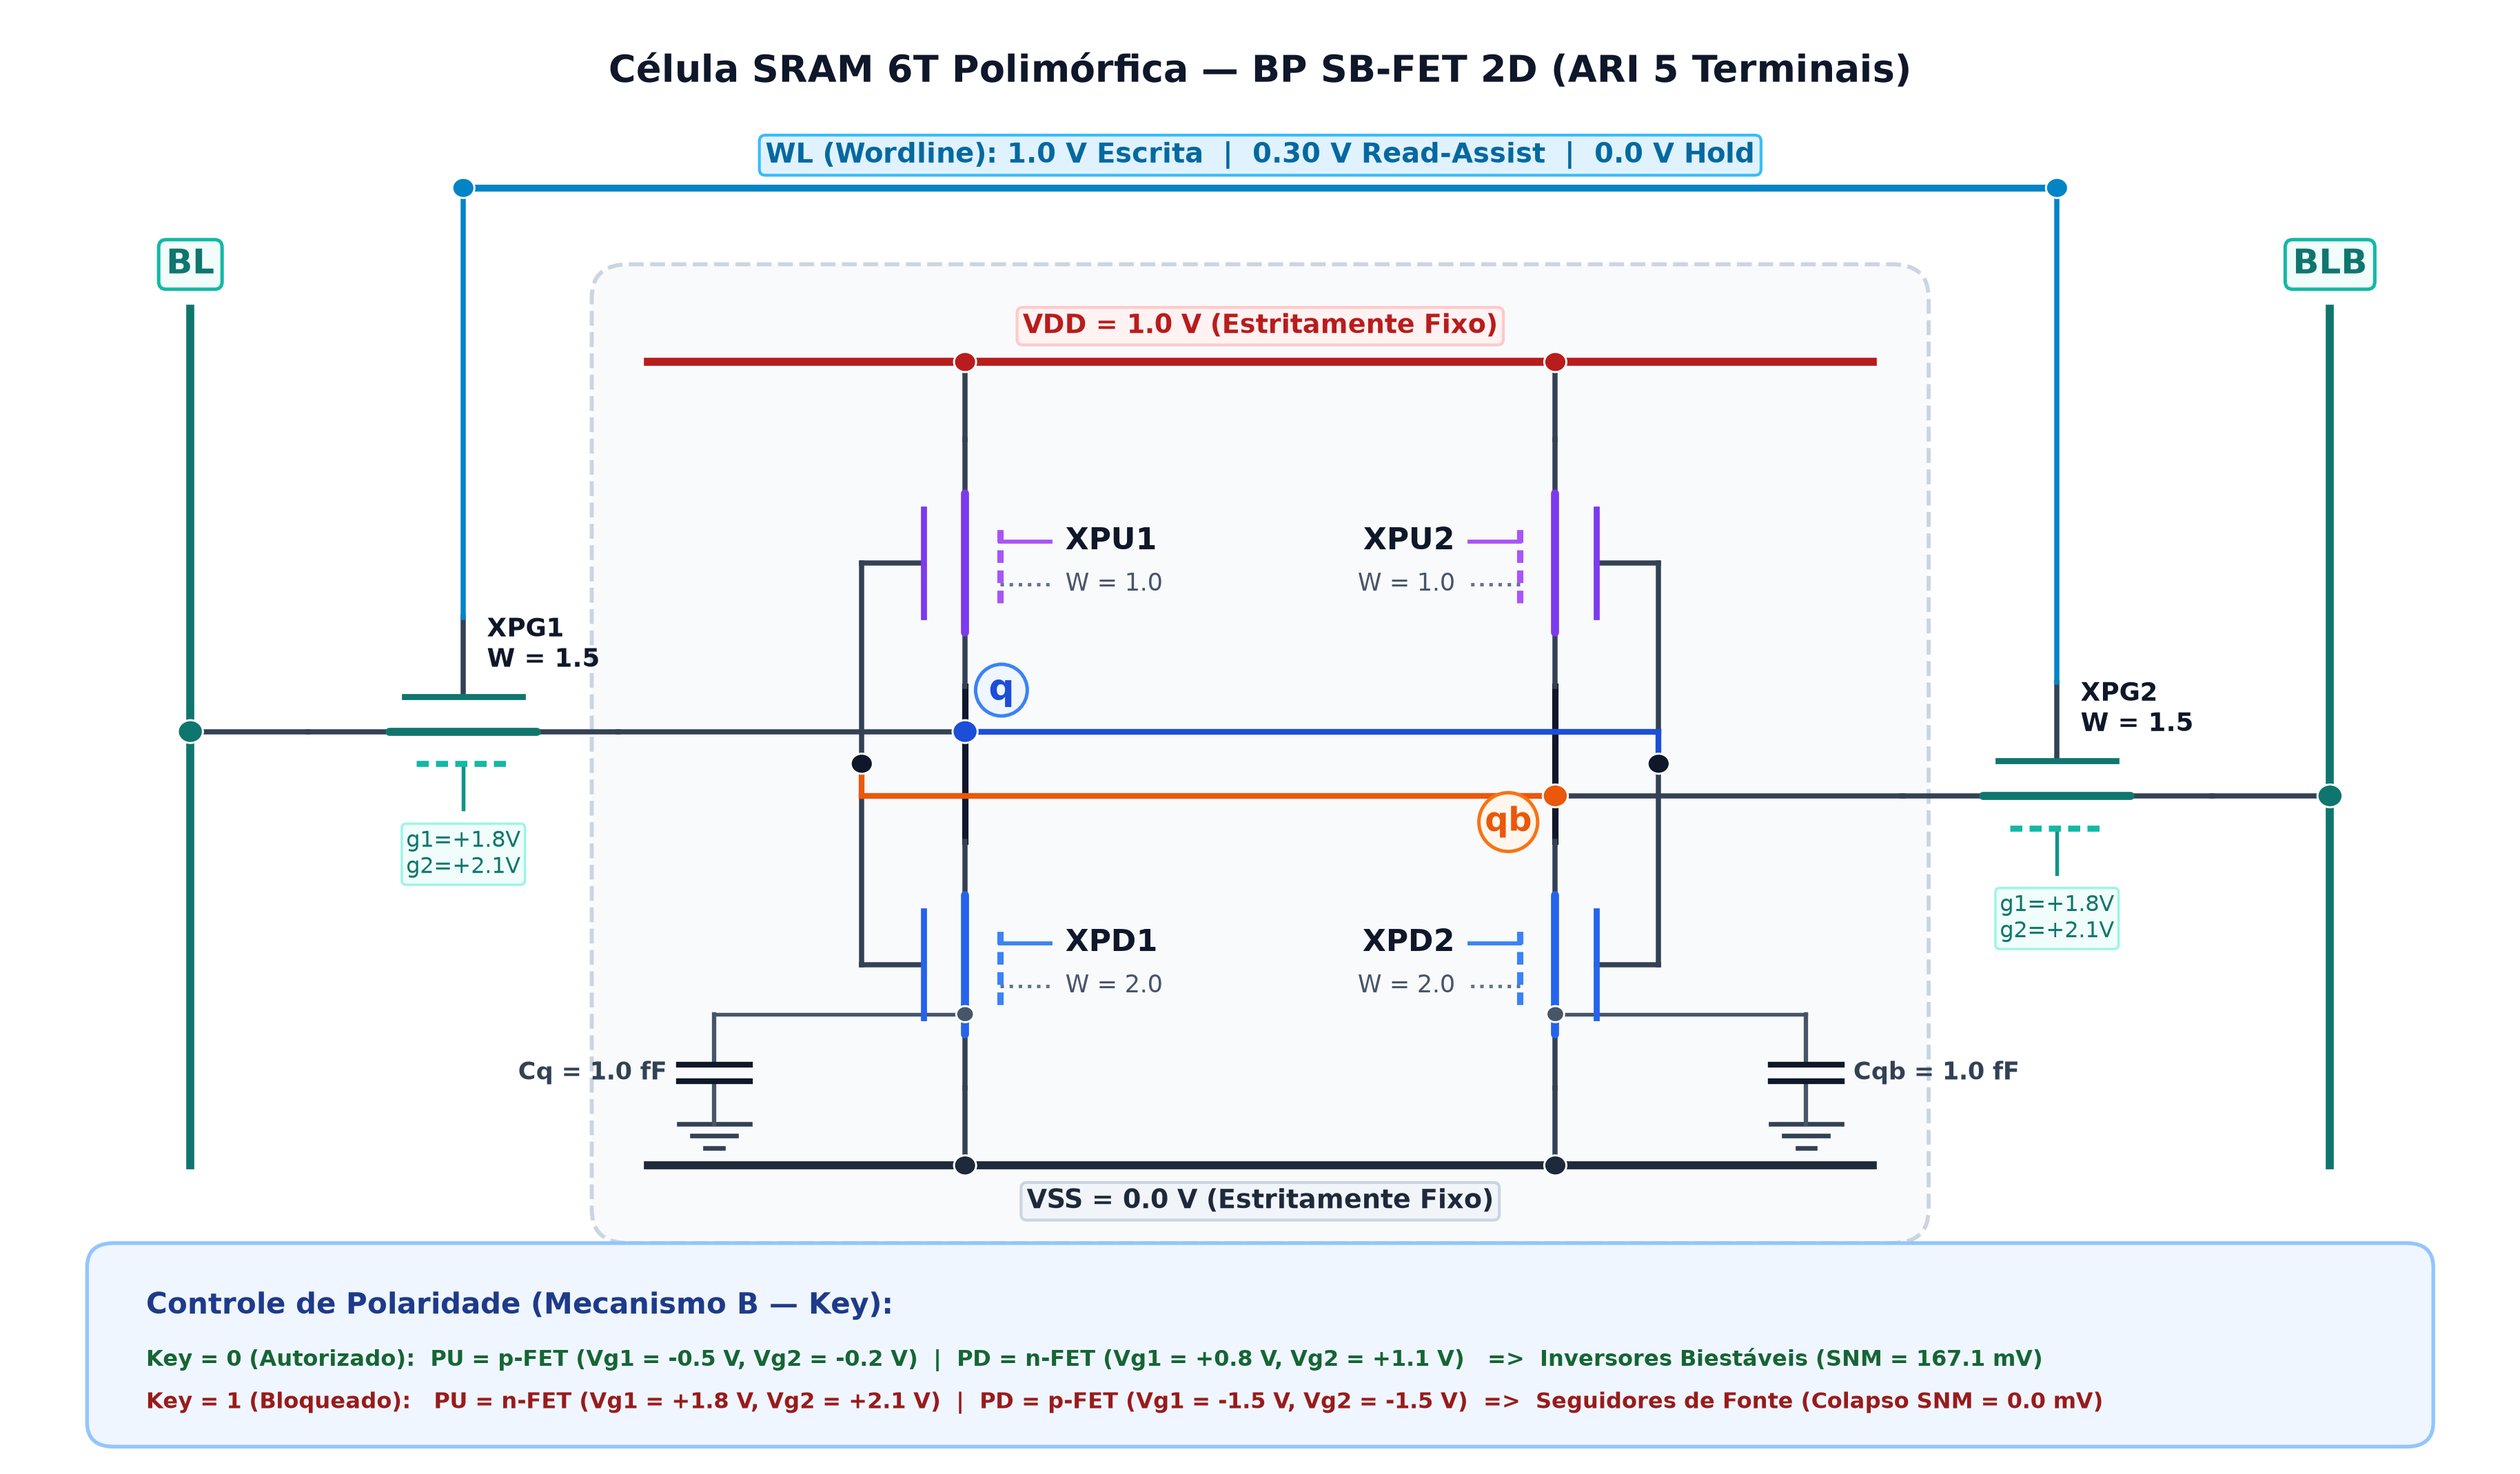
\includegraphics[width=0.98\columnwidth]{sram6t_polimorfica.png}
\caption{Schematic of the polymorphic 6T SRAM cell based on reconfigurable BP SB-FETs, illustrating fixed supply rails ($V_{DD}, V_{SS}$), storage nodes ($q, qb$), access lines ($\mathrm{WL}, \mathrm{BL}, \mathrm{BLB}$), and independent polarity-gate controls ($V_{g2,\mathrm{PU}}, V_{g2,\mathrm{PD}}, V_{g2,\mathrm{PG}}$).}
\label{fig:sram_schematic}
\end{figure}

\begin{table*}[t]
\centering
\caption{Biasing scheme of polarity-controlled retention locking (Mechanism B) in the 6T SRAM cell ($V_{DD}=1.0\ \text{V}$, $V_{SS}=0.0\ \text{V}$).}
\label{tab:sram_biases}
\footnotesize
\setlength{\tabcolsep}{4.5pt}
\begin{tabularx}{\textwidth}{>{\raggedright\arraybackslash}p{2.1cm} >{\raggedright\arraybackslash}p{3.5cm} >{\raggedright\arraybackslash}p{3.0cm} >{\raggedright\arraybackslash}p{3.0cm} >{\raggedright\arraybackslash}X}
\toprule
\textbf{Key State} & \textbf{Pull-Up ($W=1.0$)} & \textbf{Pull-Down ($W=2.0$)} & \textbf{Pass-Gates ($W=1.5$)} & \textbf{Resulting Physical Regime} \\
\midrule
$\text{Key}=0$ (Authorized) & \textit{p-FET}: $V_{g1}=-0.5\ \text{V}$, $V_{g2}=-0.2\ \text{V}$ ($V_{g2,s}=-1.2\ \text{V}$) & \textit{n-FET}: $V_{g1}=+0.8\ \text{V}$, $V_{g2}=+1.1\ \text{V}$ & \textit{n-FET}: $V_{g1}=+1.8\ \text{V}$, $V_{g2}=+2.1\ \text{V}$ & Bistable complementary CMOS inverters \\
\addlinespace[3pt]
$\text{Key}=1$ (Locked) & \textit{n-FET}: $V_{g1}=+1.8\ \text{V}$, $V_{g2}=+2.1\ \text{V}$ ($V_{g2,s}=+1.1\ \text{V}$) & \textit{p-FET}: $V_{g1}=-1.5\ \text{V}$, $V_{g2}=-1.5\ \text{V}$ & \textit{n-FET}: $V_{g1}=+1.8\ \text{V}$, $V_{g2}=+2.1\ \text{V}$ & Cross-coupled source followers (monostable collapse) \\
\bottomrule
\end{tabularx}
\end{table*}

Transient functionality and security were evaluated over a four-phase $30\ \text{ns}$ protocol:
\begin{enumerate}
    \item \textbf{Authorized Write ($0\text{--}6\ \text{ns}$, $\text{Key}=0$):} Logic \texttt{'1'} is written by asserting $\mathrm{WL} = 1.0\ \text{V}$ ($2\text{--}6\ \text{ns}$) with $\mathrm{BL} = 1.0\ \text{V}$ and $\mathrm{BLB} = 0.0\ \text{V}$.
    \item \textbf{Active Retention ($6\text{--}15\ \text{ns}$, $\text{Key}=0$):} $\mathrm{WL}$ is de-asserted ($0.0\ \text{V}$), verifying differential retention $\Delta V_{\mathrm{Key0}} = |V(q)-V(qb)| > 0.80\ \text{V}$ at $t = 12\ \text{ns}$.
    \item \textbf{Unauthorized Key Activation ($15\text{--}20\ \text{ns}$, $\text{Key}=1$):} Switching $\text{Key} \to 1$ at $t = 15\ \text{ns}$ triggers self-destruction of the stored state, verified at $t = 18\ \text{ns}$ ($\Delta V_{\mathrm{Collapse1}} < 0.15\ \text{V}$).
    \item \textbf{Locked Overwrite Attempt ($20\text{--}30\ \text{ns}$, $\text{Key}=1$):} Writing the complementary bit during $20\text{--}24\ \text{ns}$ fails to latch once $\mathrm{WL}$ closes, verified at $t = 28\ \text{ns}$ ($\Delta V_{\mathrm{Key1}} < 0.15\ \text{V}$).
\end{enumerate}

Static stability was characterized via half-cell DC butterfly sweeps ($V_{\mathrm{in}} \in [0, 1.0]\ \text{V}$, $5\ \text{mV}$ step, $\mathrm{BL} = 1.0\ \text{V}$) across six operating conditions combining $\text{Key} \in \{0, 1\}$ and $\mathrm{WL} \in \{0.0\ \text{V}\ (\text{Hold}),\ 0.30\ \text{V}\ (\text{Wordline Underdrive Read-Assist}),\ 1.0\ \text{V}\ (\text{Unassisted Read})\}$. The SNM was extracted geometrically over a 2,000-point grid in the $45^\circ$-rotated coordinate frame:
\begin{align}
u &= \frac{V_{qb} - V_q}{\sqrt{2}}, \qquad v = \frac{V_{qb} + V_q}{\sqrt{2}}, \nonumber \\
\mathrm{SNM} &= \max_{u < 0} \frac{v_1(u) - v_2(u)}{\sqrt{2}}. \label{eq:snm_45}
\end{align}

\section{Results and Discussion}
\subsection{4D BP SB-FET Model Validation and Flat-Band Behavior}
At $|V_{ds}| = 0.8\ \text{V}$, \texttt{bp\_ari\_\allowbreak ngspice.lib} (\texttt{v2}) reproduced the experimental lookup tables with mean relative errors of $0.0621\%$ in \textit{n-FET} mode ($I_{\mathrm{on}} = 1.650\ \mu\text{A}/\mu\text{m}$, $I_{\mathrm{off}} = 0.596\ \text{nA}/\mu\text{m}$, $I_{\mathrm{on}}/I_{\mathrm{off}} = 2.77 \times 10^3$, $SS_{\min} = 106.59\ \text{mV/dec}$ at $V_{g1}=1.1\ \text{V}, V_{g2}=0.8\ \text{V}$) and $0.0032\%$ in \textit{p-FET} mode ($I_{\mathrm{on}} = 1.790\ \mu\text{A}/\mu\text{m}$, $I_{\mathrm{off}} = 2.811\ \text{nA}/\mu\text{m}$, $I_{\mathrm{on}}/I_{\mathrm{off}} = 6.37 \times 10^2$, $SS_{\min} = 148.08\ \text{mV/dec}$ at $V_{g1}=-1.5\ \text{V}, V_{g2}=-1.2\ \text{V}$).

Table~\ref{tab:hspice_validation} and Fig.~\ref{fig:m00_hspice} summarize the quantitative cross-validation against Synopsys HSPICE \texttt{.printtr0} reference outputs. While transfer curves attained $R^2 \ge 0.99994$ in both versions, incorporating the measured $V_{g2} = -1.5\ \text{V}$ surface in \texttt{v2} reduced \texttt{P\_output} RMSE by $99.5\%$ (\textbf{$196\times$}, from $0.590087$ to $0.003013\ \mu\text{A}/\mu\text{m}$, raising $R^2$ from $-7.6723$ to $0.999774$) and lowered \texttt{N\_output} RMSE by $33.6\%$ ($R^2 = 0.927855$). As illustrated in Fig.~\ref{fig:m00_pg}, electrostatic modulation by $V_{g2}$ exhibits a pronounced flat-band shift ($\Delta V_{fb} \approx -0.25\ \text{V}$) at $V_{g2} = -1.5\ \text{V}$, directly governing the pull-up drive strength of the 6T SRAM cell.

\begin{table}[t]
\centering
\caption{Quantitative cross-validation between \texttt{ngspice-47} (\texttt{v1} and \texttt{v2}) and Synopsys HSPICE \texttt{.printtr0} outputs (RMSE in $\mu\text{A}$).}
\label{tab:hspice_validation}
\scriptsize
\setlength{\tabcolsep}{3pt}
\begin{tabularx}{\columnwidth}{>{\raggedright\arraybackslash}X c c c c}
\toprule
\textbf{Regime} & $\text{RMSE}_{\mathrm{v1}}$ & $\text{RMSE}_{\mathrm{v2}}$ & \textbf{Red.} & $R^2_{\mathrm{v2}}$ \\
\midrule
\texttt{N\_transfer} & $0.001910$ & $0.001899$ & $-0.6\%$ & $0.999972$ \\
\texttt{P\_transfer} & $0.000947$ & $0.000947$ & $0.0\%$ & $0.999944$ \\
\texttt{N\_output} & $0.196416$ & $0.130430$ & $-33.6\%$ & $0.927855$ \\
\texttt{P\_out} ($-1.5\,$V) & $0.590087$ & $0.003013$ & $-99.5\%$ & $0.999774$ \\
\bottomrule
\end{tabularx}
\end{table}

\begin{figure}[t]
\centering
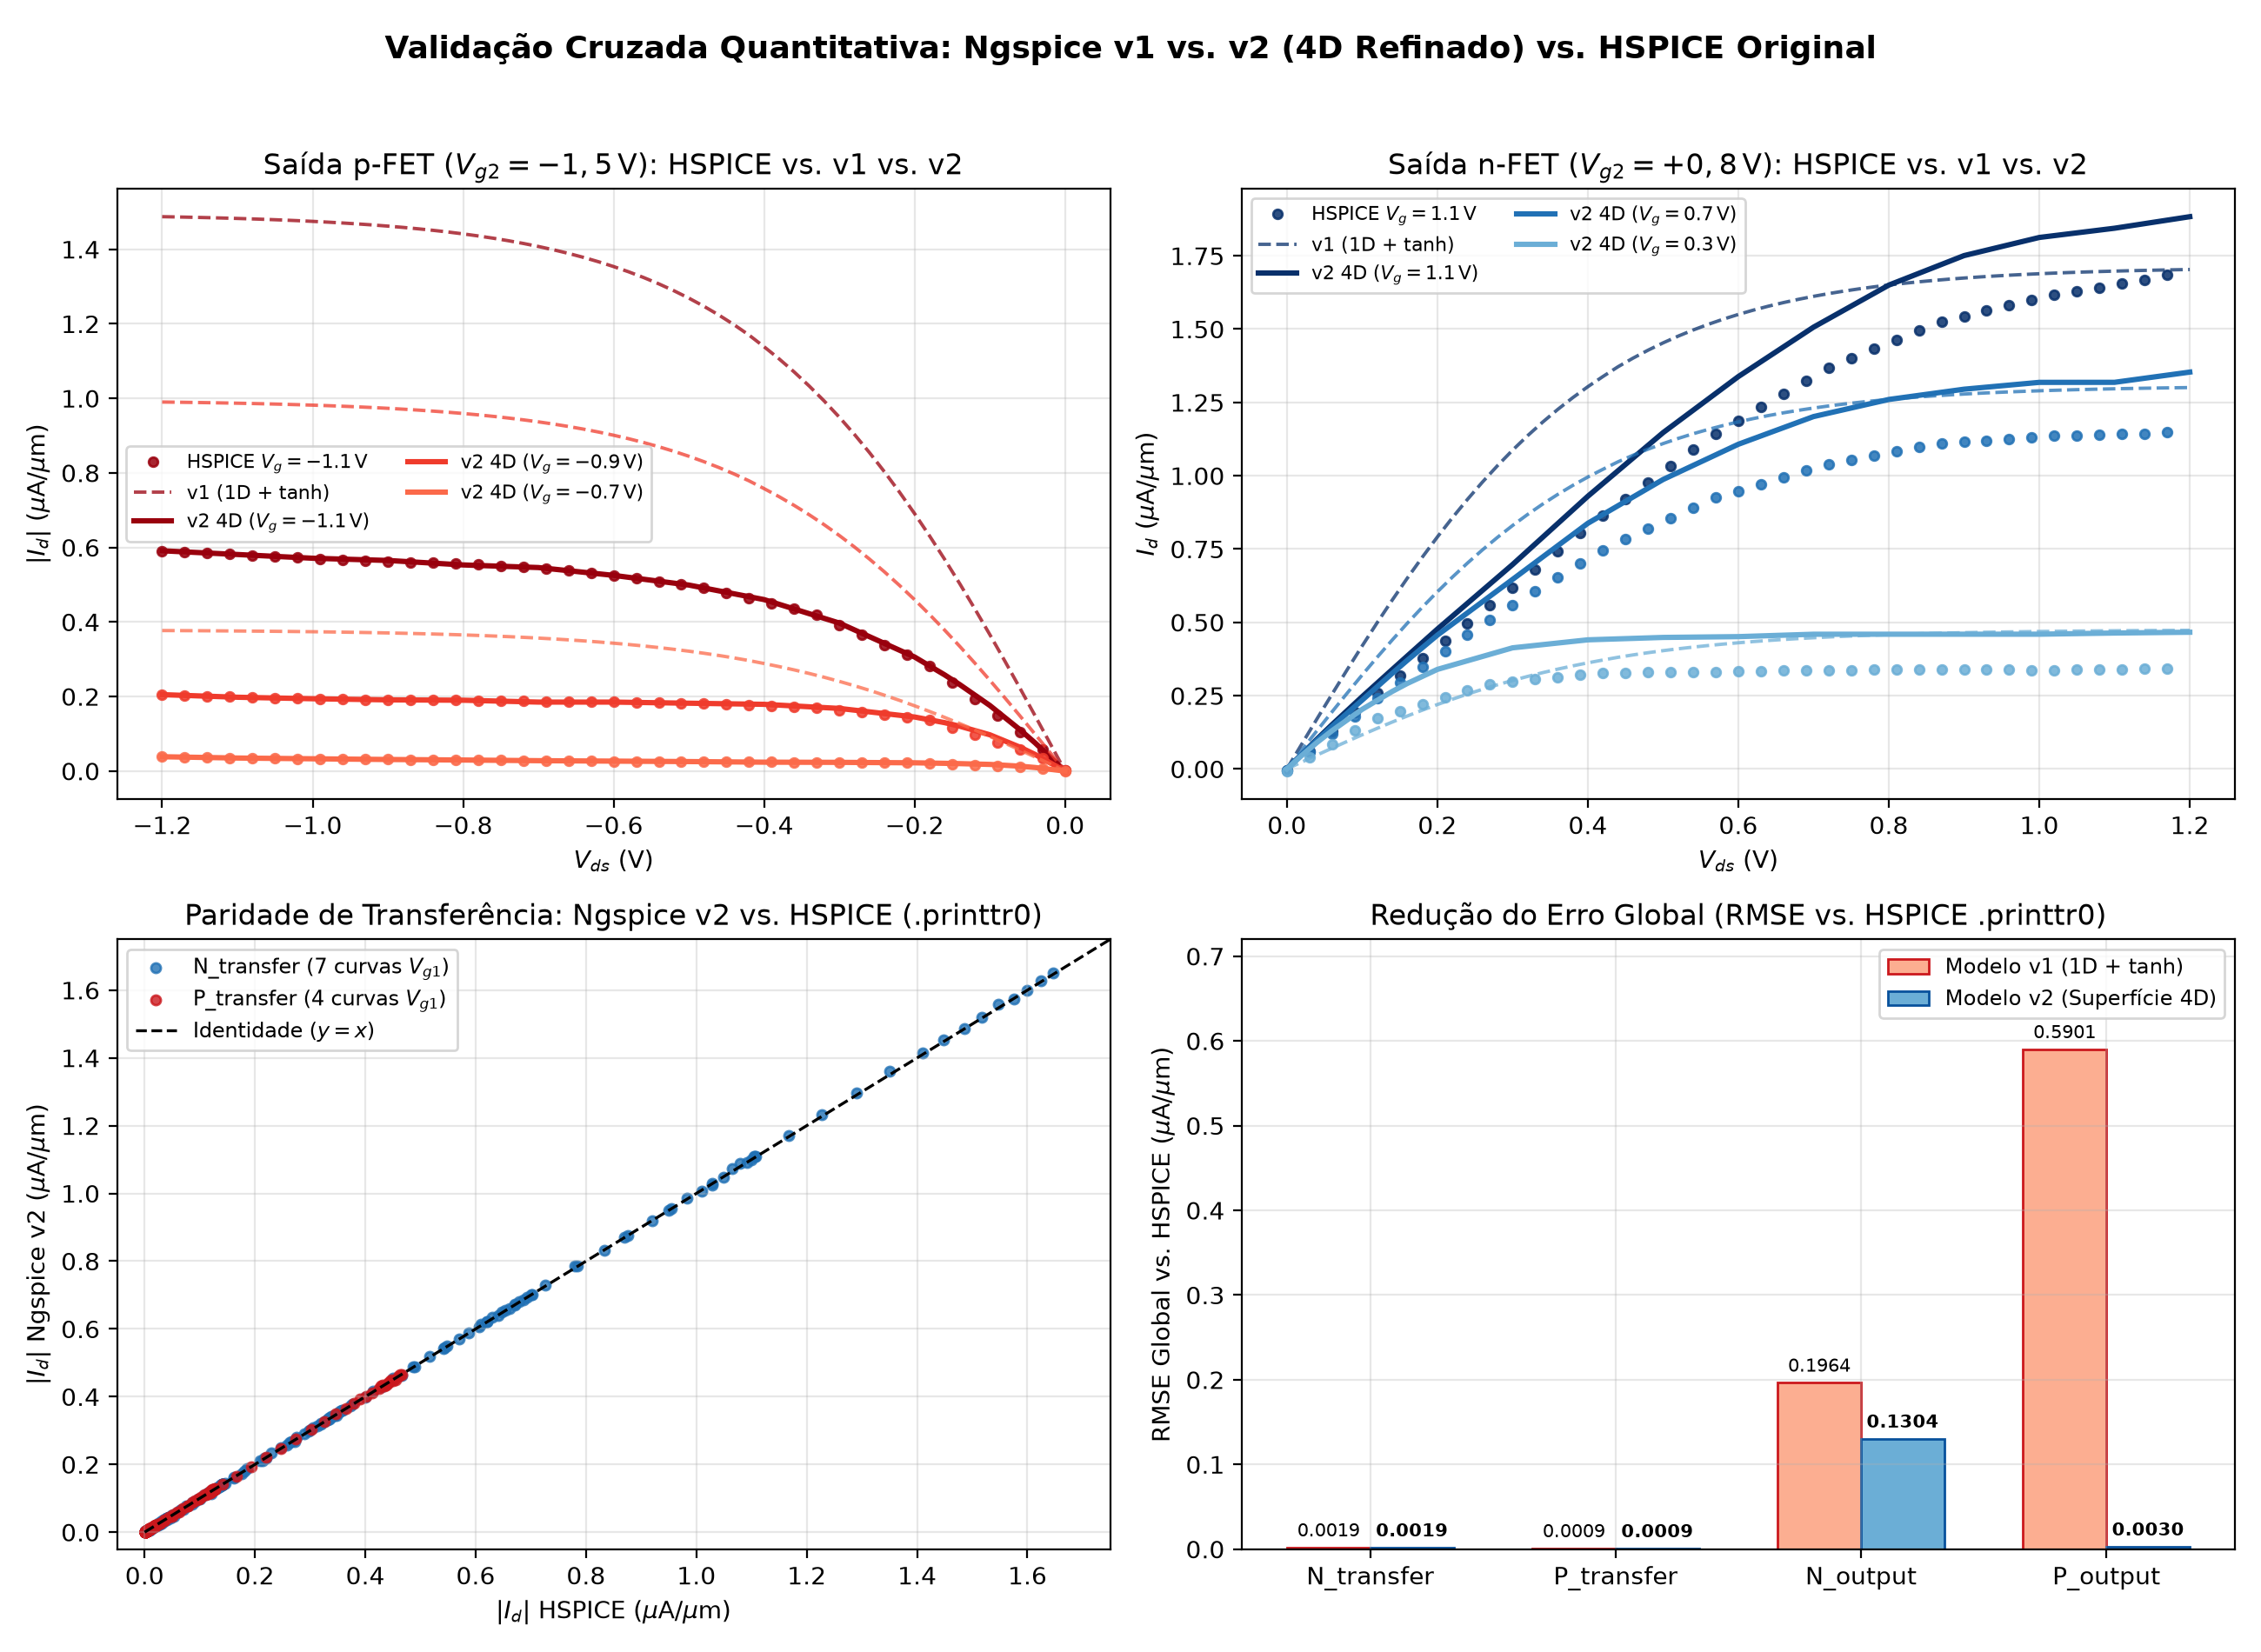
\includegraphics[width=0.98\columnwidth]{m00_validacao_cruzada_hspice.png}
\caption{Cross-validation comparing the preliminary 1D model (\texttt{v1}), the refined 4D model (\texttt{v2}) in \texttt{ngspice-47}, and Synopsys HSPICE \texttt{.printtr0} reference outputs.}
\label{fig:m00_hspice}
\end{figure}

\begin{figure}[t]
\centering
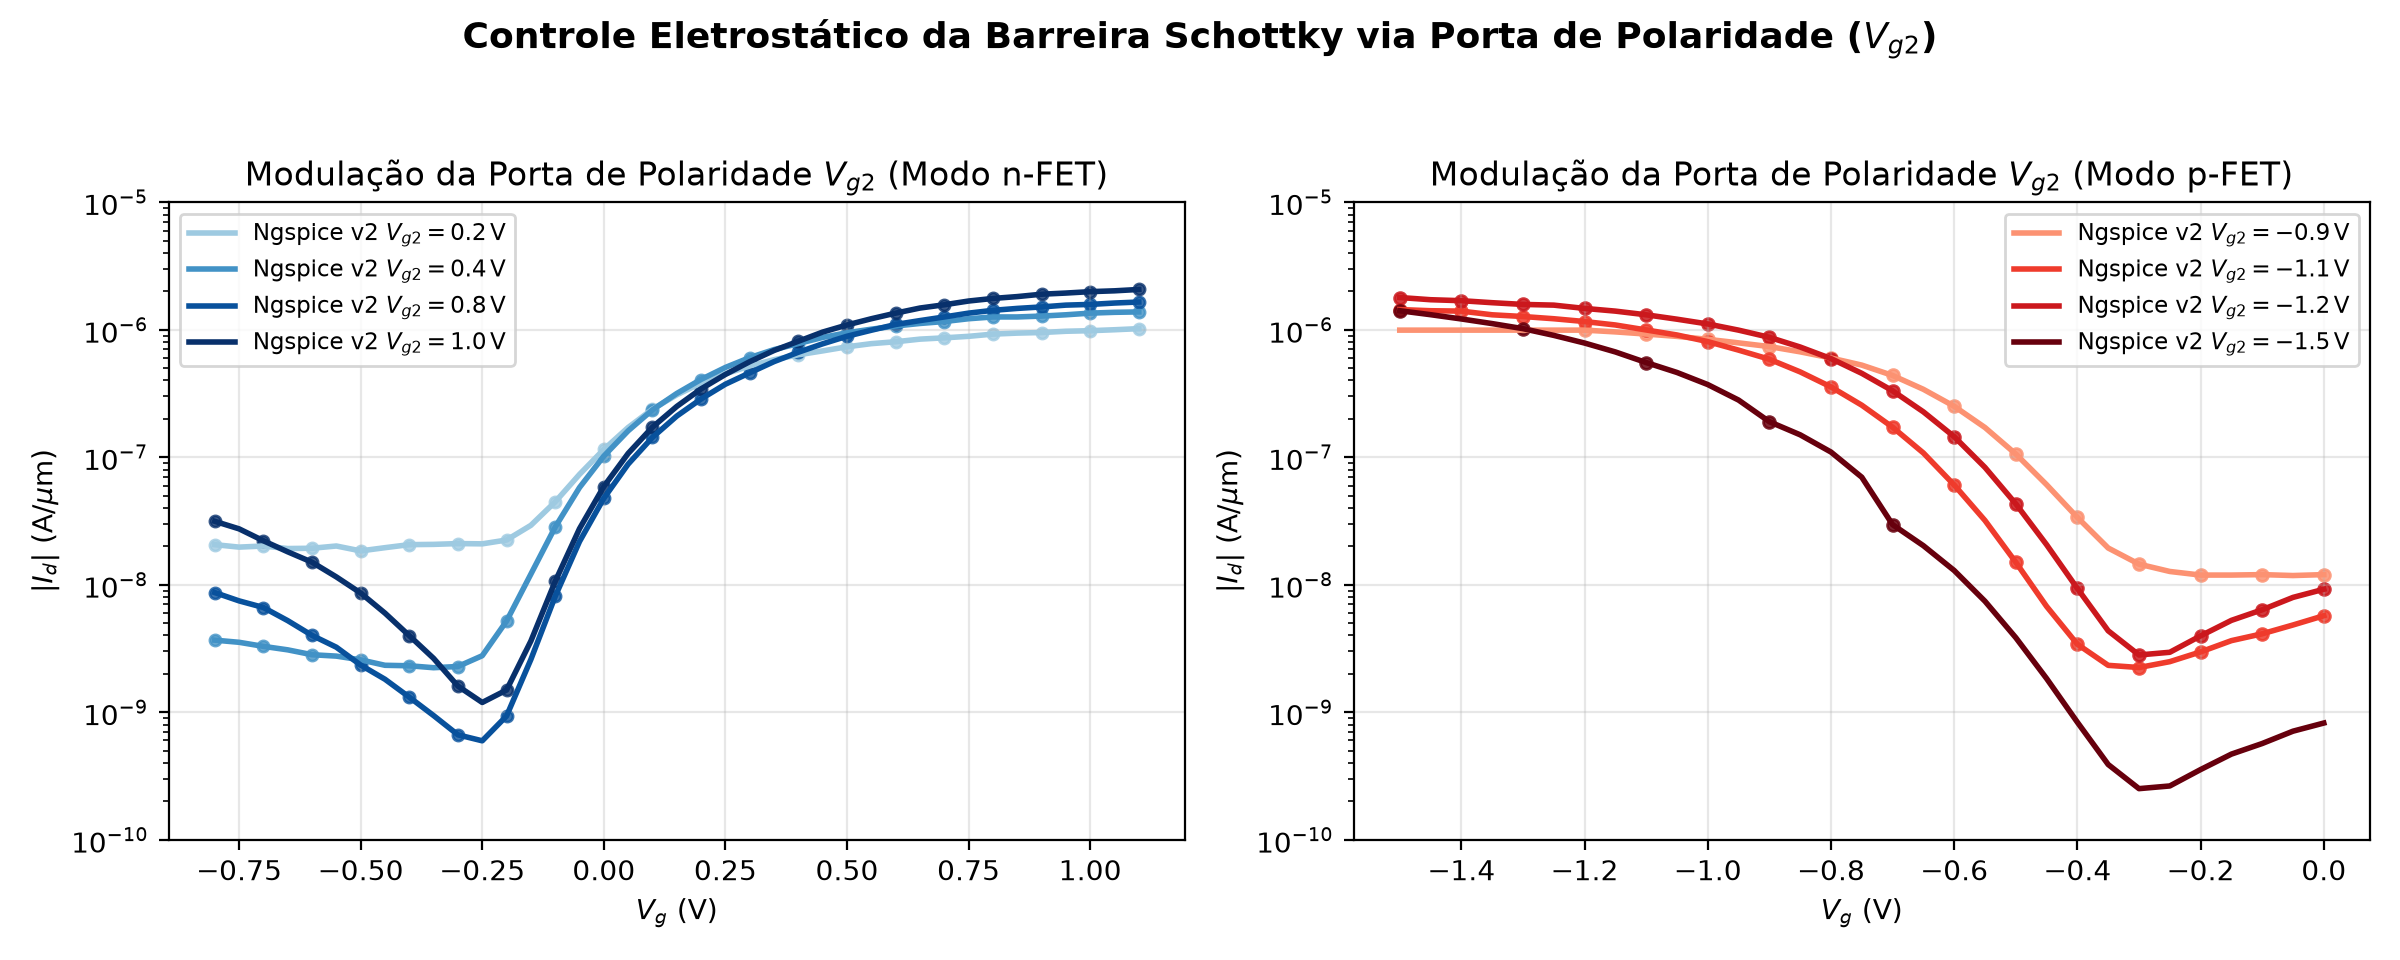
\includegraphics[width=0.98\columnwidth]{m00_efeito_porta_polaridade.png}
\caption{Electrostatic modulation of drain current by the polarity gate $V_{g2}$ in \textit{n-FET} and \textit{p-FET} modes, highlighting the flat-band shift at $V_{g2}=-1.5\ \text{V}$.}
\label{fig:m00_pg}
\end{figure}

\subsection{Transient Retention Locking and Self-Destruction in the 6T SRAM}
The polymorphic 6T SRAM cell satisfied all eleven transient and static acceptance criteria for \textit{Mechanism B}, as compiled in Table~\ref{tab:sram_results}. During the $30\ \text{ns}$ transient simulation (Fig.~\ref{fig:m04_tran}), under $\text{Key}=0$, the logic \texttt{'1'} written in Phase~1 ($0\text{--}6\ \text{ns}$) is stably retained after wordline de-assertion, reaching $V(q) = 0.9768\ \text{V}$ and $V(qb) = 0.0020\ \text{V}$ at $t = 12\ \text{ns}$ ($\Delta V_{\mathrm{Key0}} = 0.9747\ \text{V} > 0.80\ \text{V}$).

\begin{table}[t]
\centering
\caption{Transient ($30\ \text{ns}$) and static noise margin (SNM) metrics of the polymorphic 6T SRAM cell.}
\label{tab:sram_results}
\scriptsize
\setlength{\tabcolsep}{2.5pt}
\begin{tabularx}{\columnwidth}{>{\raggedright\arraybackslash}X c >{\raggedright\arraybackslash}p{2.15cm}}
\toprule
\textbf{Extracted Metric} & \textbf{Sim.} & \textbf{Criterion / Status} \\
\midrule
$V(q)_{\mathrm{Hold}}$ ($\text{Key}=0,\ 12\,$ns) & $0.9768\,$V & $> 0.80\,$V (Passed) \\
$V(qb)_{\mathrm{Hold}}$ ($\text{Key}=0,\ 12\,$ns) & $0.0020\,$V & $< 0.20\,$V (Passed) \\
$\Delta V_{\mathrm{Key0}}$ ($12\,$ns) & $0.9747\,$V & $> 0.80\,$V (Passed) \\
$\Delta V_{\mathrm{Collapse1}}$ ($18\,$ns) & $0.0841\,$V & $< 0.15\,$V (Passed) \\
$\Delta V_{\mathrm{Key1}}$ ($28\,$ns) & $0.0762\,$V & $< 0.15\,$V (Passed) \\
$\mathrm{SNM}_{\mathrm{Hold}}$ ($\text{Key}=0,\ \mathrm{WL}=0\,$V) & $167.12\,$mV & $> 150\,$mV (Passed) \\
$\mathrm{SNM}_{\mathrm{Read,Unass.}}$ ($\mathrm{WL}=1.0\,$V) & $0.00\,$mV & \textit{Read Disturb} \\
$\mathrm{SNM}_{\mathrm{Read,Assist}}$ ($\mathrm{WL}=0.30\,$V) & $66.23\,$mV & $> 50\,$mV (Passed) \\
$\mathrm{SNM}_{\mathrm{Hold}}$ ($\text{Key}=1,\ \mathrm{WL}=0\,$V) & $0.00\,$mV & $= 0\,$mV (Locked) \\
$\mathrm{SNM}_{\mathrm{Read,Assist}}$ ($\text{Key}=1,\ 0.30\,$V) & $0.00\,$mV & $= 0\,$mV (Locked) \\
$\mathrm{SNM}_{\mathrm{Read,Unass.}}$ ($\text{Key}=1,\ 1.0\,$V) & $0.00\,$mV & $= 0\,$mV (Locked) \\
\bottomrule
\end{tabularx}
\end{table}

When the security key switches to $\text{Key}=1$ at $t = 15\ \text{ns}$ (Phase~3)---while keeping $V_{DD} = 1.0\ \text{V}$ and $V_{SS} = 0.0\ \text{V}$ completely constant---simultaneous polarity inversion of the pull-up (\textit{p-FET} $\to$ \textit{n-FET}) and pull-down (\textit{n-FET} $\to$ \textit{p-FET}) devices eliminates regenerative feedback. Both internal nodes rapidly converge toward a monostable equilibrium, collapsing the differential stored voltage by more than $91\%$ within $3\ \text{ns}$ ($\Delta V_{\mathrm{Collapse1}} = 0.0841\ \text{V} < 0.15\ \text{V}$ at $t = 18\ \text{ns}$). Furthermore, in Phase~4 ($20\text{--}30\ \text{ns}$), even when an adversary forces opposite bitline potentials while $\mathrm{WL} = 1.0\ \text{V}$ is asserted, the cell collapses immediately upon wordline turn-off ($\Delta V_{\mathrm{Key1}} = 0.0762\ \text{V}$ at $t = 28\ \text{ns}$), preventing unauthorized data injection while locked.

\begin{figure}[t]
\centering
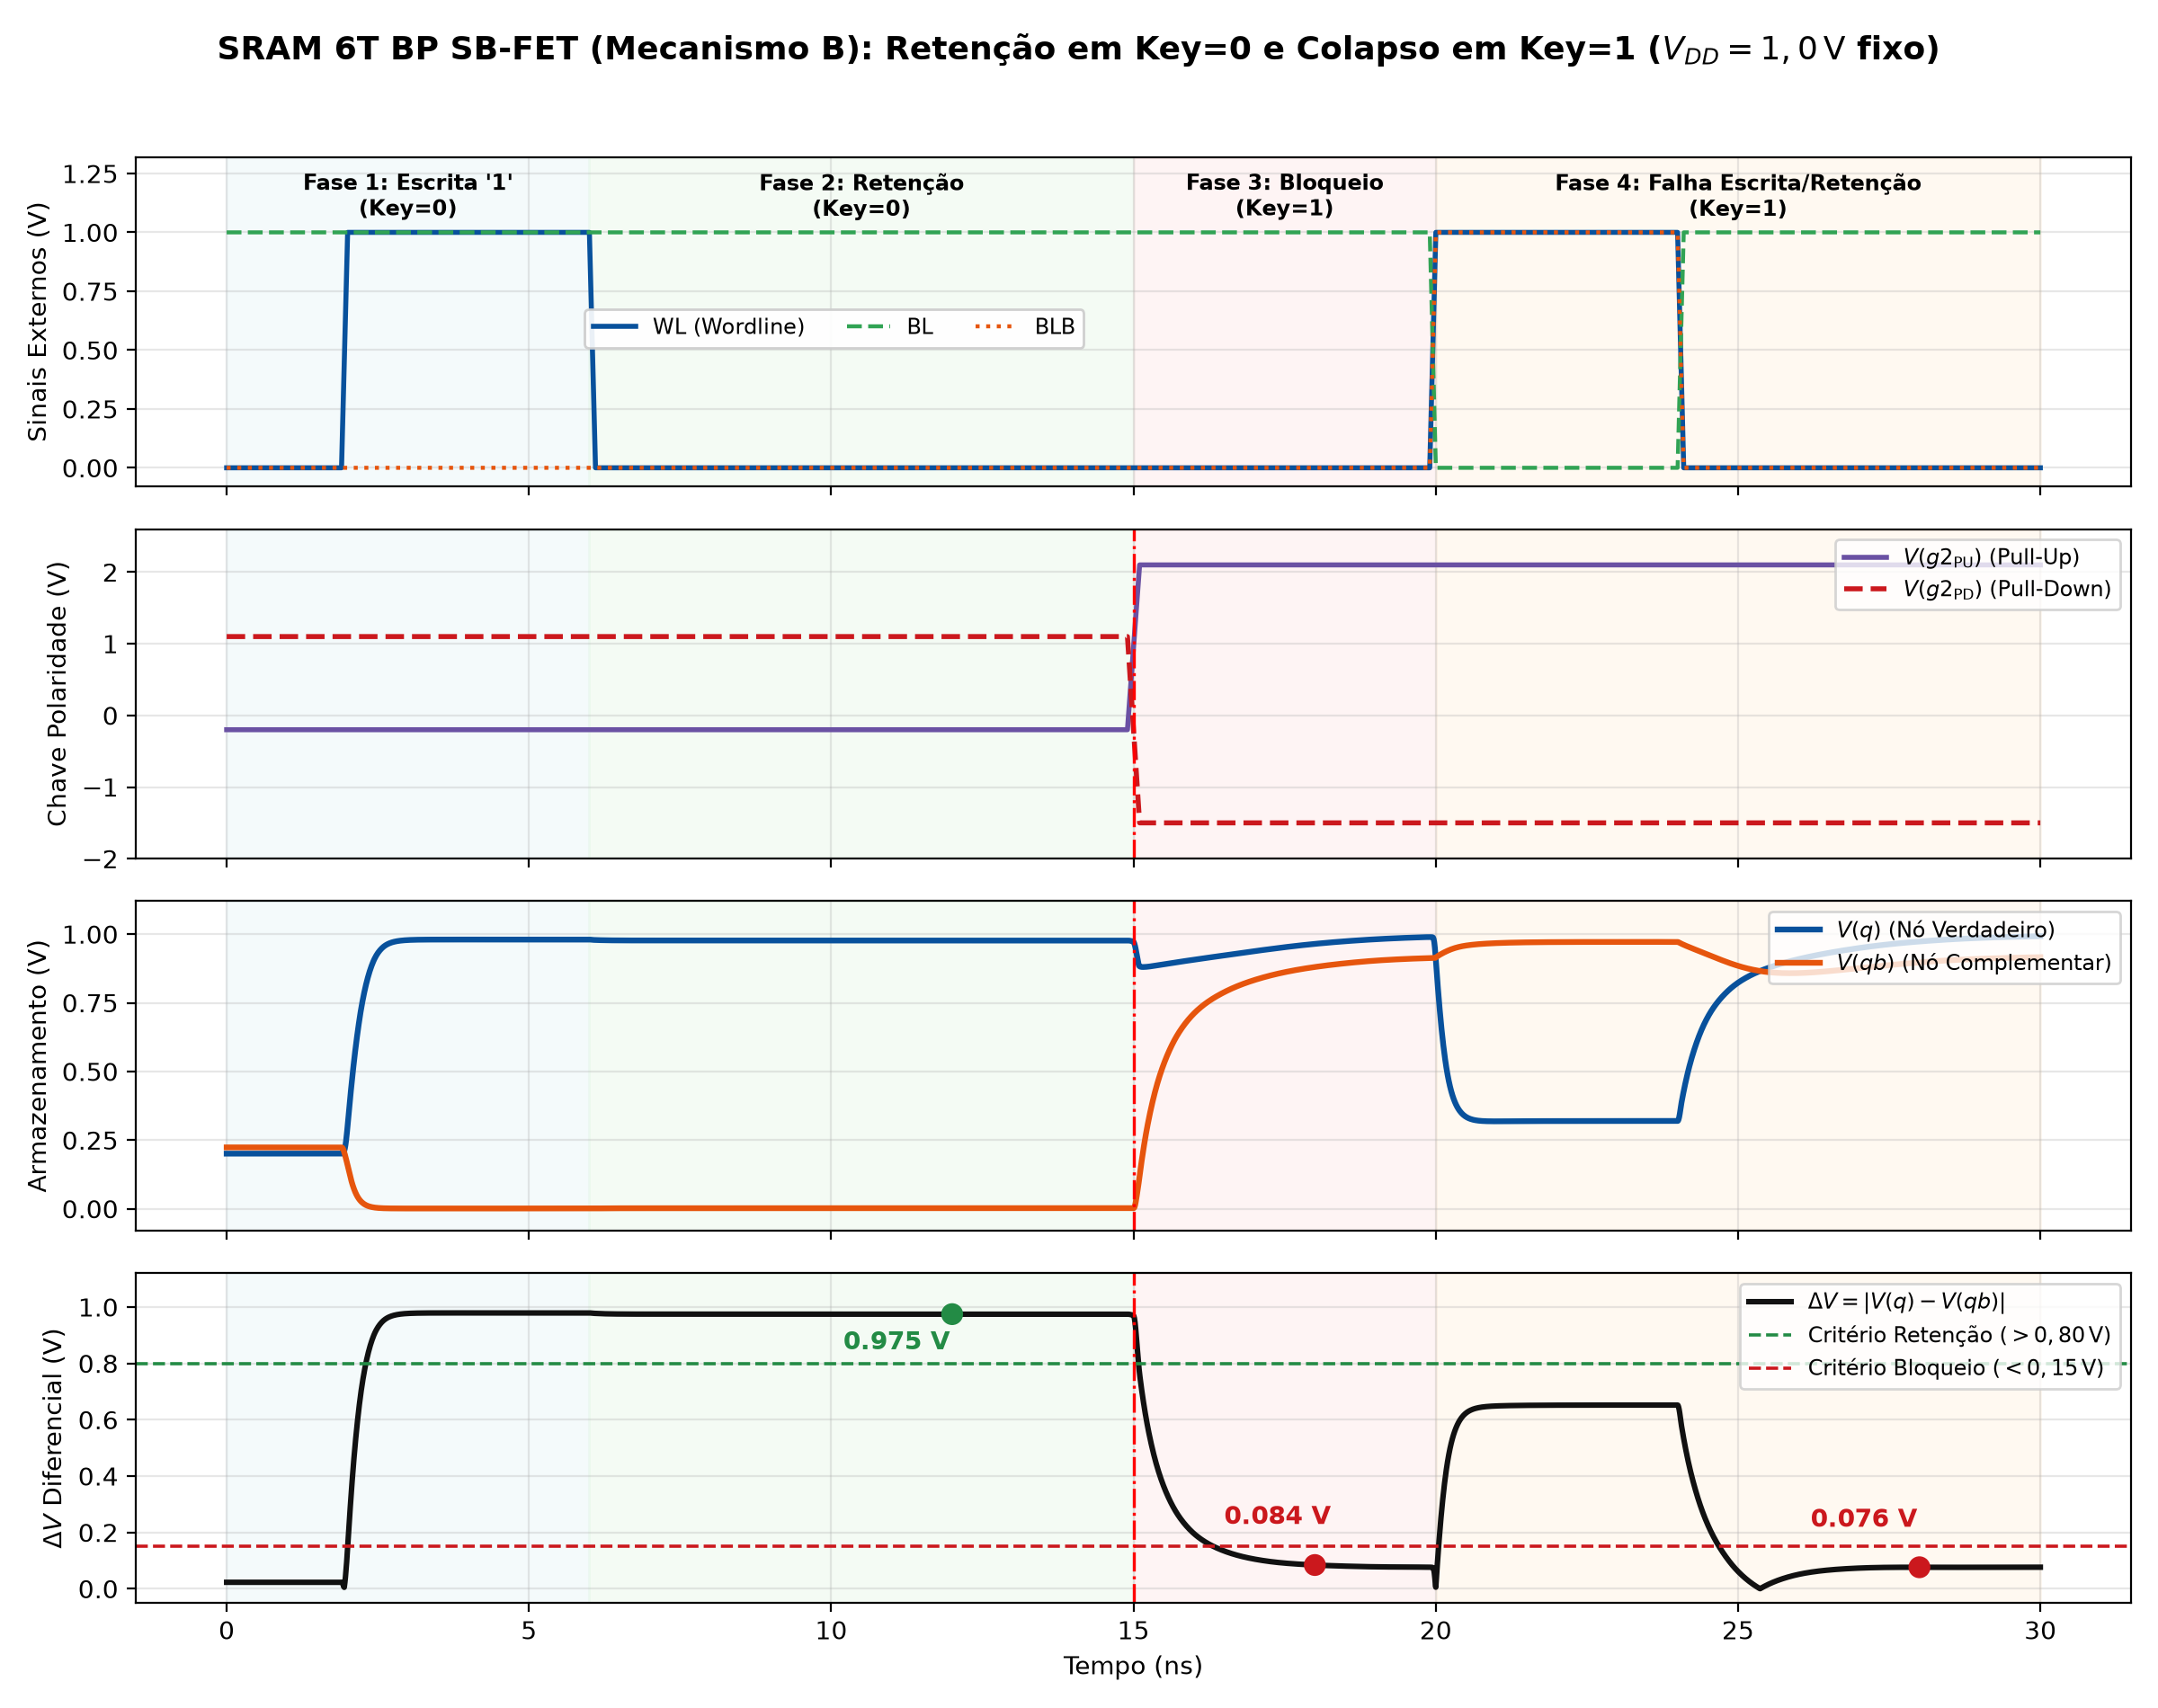
\includegraphics[width=0.98\columnwidth]{m04_sram_transiente_30ns.png}
\caption{Four-phase $30\ \text{ns}$ transient simulation of the polymorphic 6T SRAM cell: write and stable retention under $\text{Key}=0$ ($0\text{--}15\ \text{ns}$) followed by state collapse and rewrite immunity under $\text{Key}=1$ ($15\text{--}30\ \text{ns}$).}
\label{fig:m04_tran}
\end{figure}

\subsection{Butterfly-Curve SNM Analysis and Read-Assist Mitigation}
Static butterfly-curve analysis (Fig.~\ref{fig:m04_snm}) yielded two critical physical design insights for 2D BP SB-FET memories:
\begin{enumerate}
    \item \textbf{Flat-Band Polarity Tuning:} Under an unoptimized pull-up bias of $V_{g2,\mathrm{PU}} = -0.5\ \text{V}$ ($V_{g2,s} = -1.5\ \text{V}$), the $\Delta V_{fb} \approx -0.25\ \text{V}$ shift captured by our 4D model reduces \textit{p-FET} drive current from $1.79$ to $0.37\ \mu\text{A}$ (at $V_{gp} = -1.0\ \text{V}$), skewing the inverter switching threshold and degrading $\mathrm{SNM}_{\mathrm{Hold}}$ to $49.4\ \text{mV}$. Adjusting $V_{g2,\mathrm{PU}}$ to $-0.2\ \text{V}$ ($V_{g2,s} = -1.2\ \text{V}$) restores pull-up/pull-down symmetry without increasing transistor widths, achieving $\mathrm{SNM}_{\mathrm{Hold}} = 167.12\ \text{mV}$ ($16.7\%$ of $V_{DD}$).
    \item \textbf{Read Disturb Mitigation via Wordline Underdrive:} During unassisted read access ($\text{Key}=0, \mathrm{WL}=1.0\ \text{V}$), strong access pass-gates ($W_{\mathrm{PG}} = 1.5$) pull the low storage node above the trip point, causing destructive \textit{Read Disturb} ($\mathrm{SNM}_{\mathrm{Read,Unassisted}} = 0.00\ \text{mV}$). Applying \textit{Wordline Underdrive Read-Assist} at $\mathrm{WL} = 0.30\ \text{V}$ weakens pass-gate contention during read cycles and restores a stable noise margin of $\mathrm{SNM}_{\mathrm{Read,Assist}} = 66.23\ \text{mV}$, whereas all $\text{Key}=1$ regimes remain strictly locked at $\mathrm{SNM} = 0.00\ \text{mV}$ (single intersection point in Fig.~\ref{fig:m04_snm}, right).
\end{enumerate}

\begin{figure}[t]
\centering
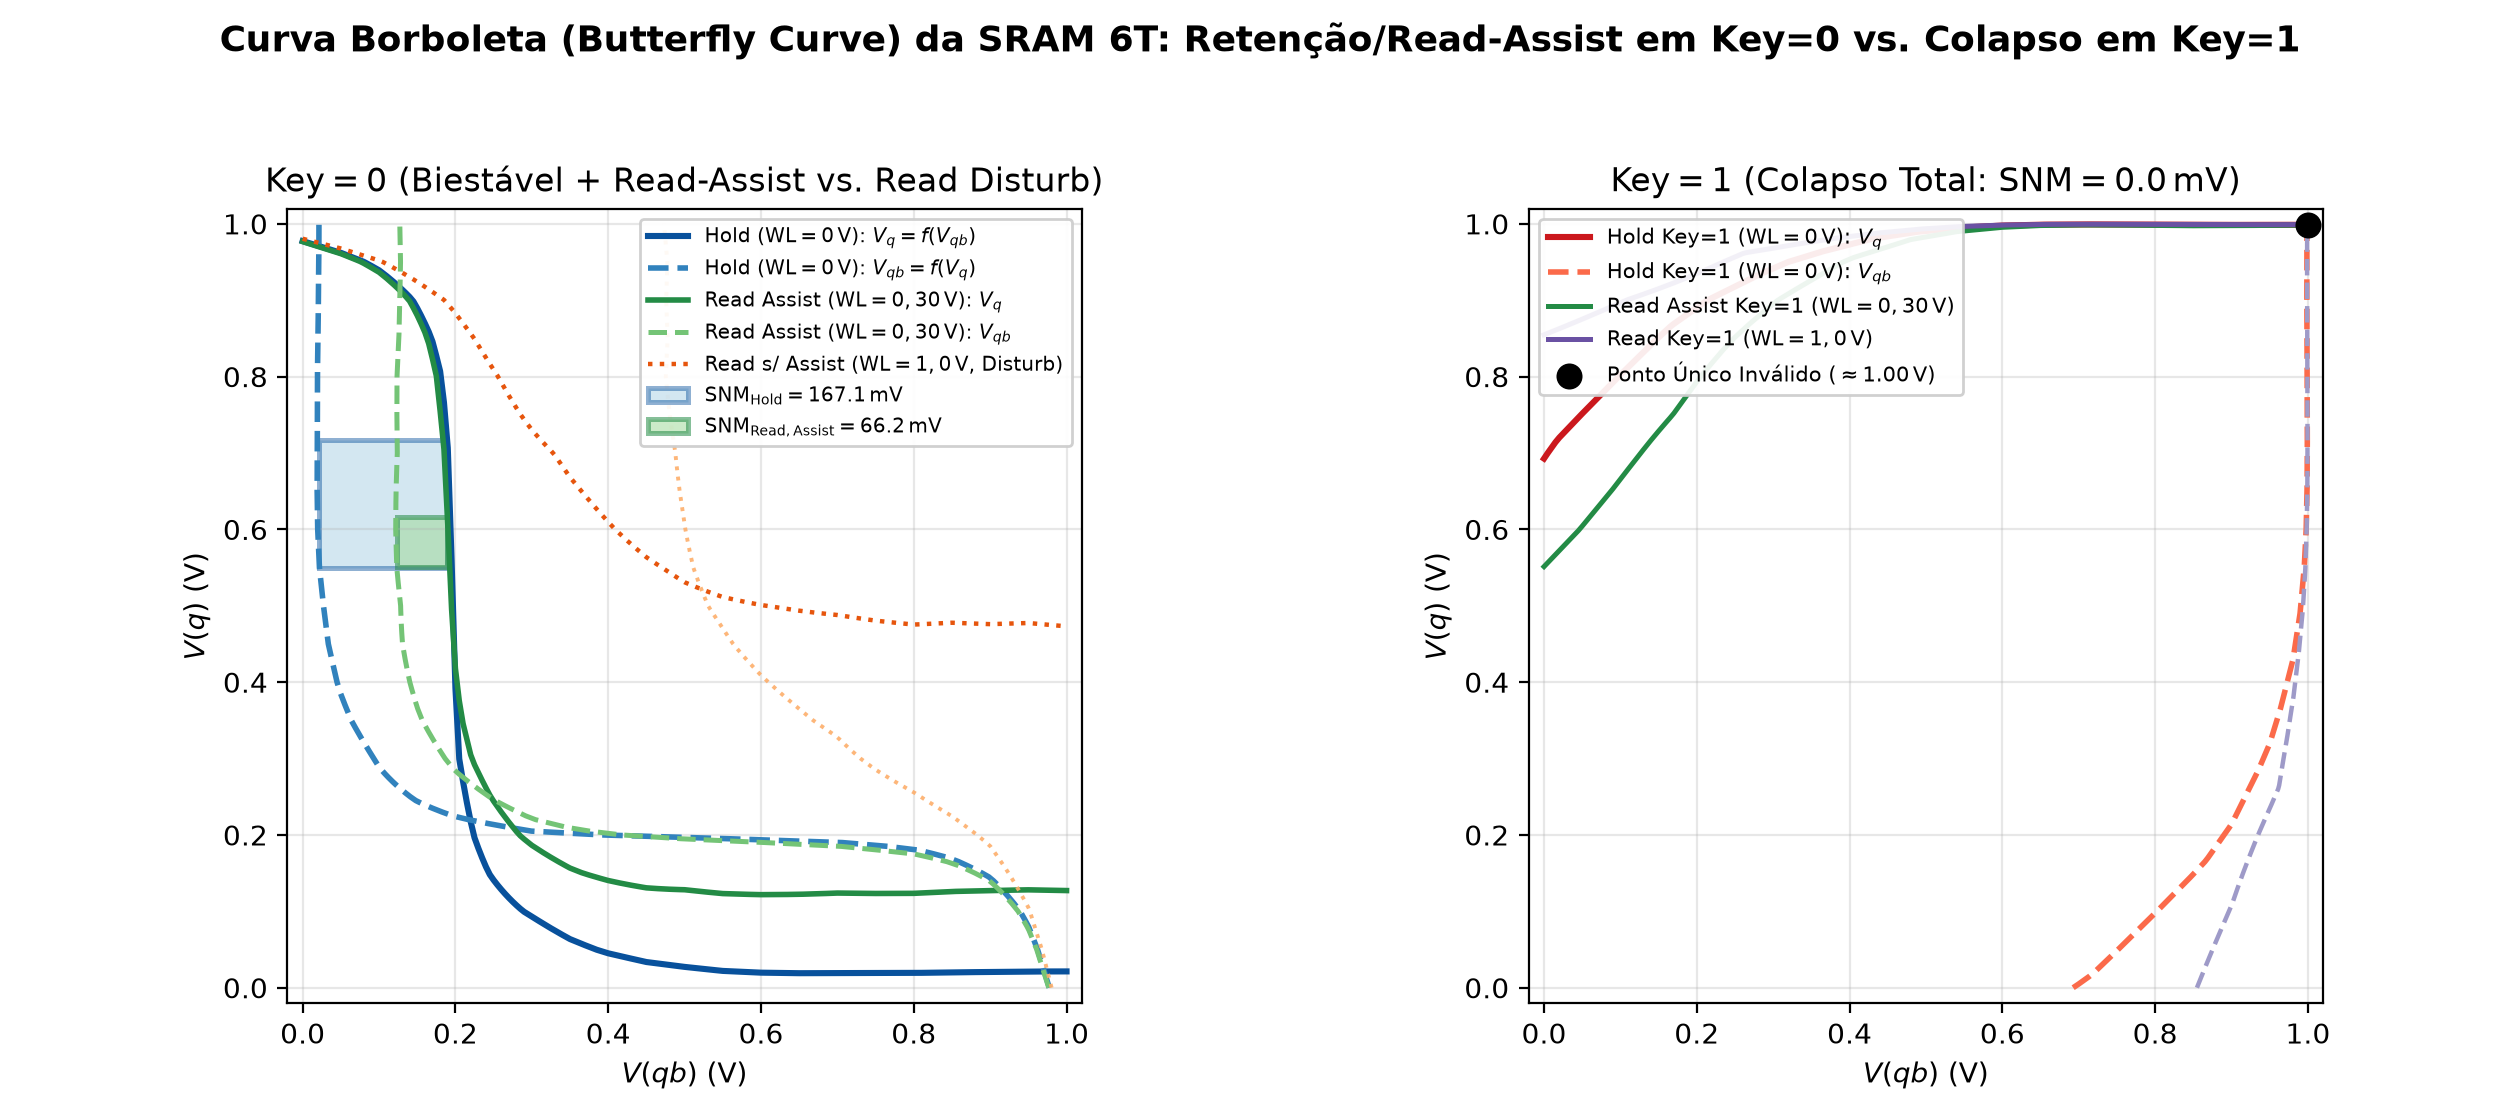
\includegraphics[width=0.98\columnwidth]{m04_sram_curva_borboleta_snm.png}
\caption{6T SRAM butterfly curves and maximum inscribed SNM squares for $\text{Key}=0$ (Hold, Wordline Read-Assist, and Unassisted Read showing \textit{Read Disturb}) versus monostable collapse at $\text{Key}=1$ ($\mathrm{SNM}=0.00\ \text{mV}$).}
\label{fig:m04_snm}
\end{figure}

From a hardware security perspective, \textit{Mechanism B} offers distinct advantages over conventional CMOS zeroization: (i)~instantaneous data erasure occurs within $<3\ \text{ns}$ via low-capacitance polarity gates while $V_{DD}$ and $V_{SS}$ remain constant, defeating supply-clamping tamper attacks; (ii)~the physical cell layout is identical to a standard 6T topology with zero extra transistors; and (iii)~key removal renders the memory array incapable of holding state even under active write stimuli.

\section{Conclusion}
This work presented the modeling, circuit design, and security evaluation of a polymorphic 6T SRAM cell using ambipolar 2D BP SB-FETs in an open-source \texttt{ngspice-47} and Python environment. Translating 4D experimental lookup tables with bilateral source referencing and gate-specific saturation curves (\texttt{bp\_ari\_\allowbreak ngspice.lib} \texttt{v2}) reproduced experimental characteristics within $0.0621\%$ mean error and reduced \textit{p-FET} output RMSE against Synopsys HSPICE by $196\times$ by explicitly capturing the $V_{g2}=-1.5\ \text{V}$ flat-band regime. In the 6T SRAM cell, polarity-controlled retention locking (\textit{Mechanism B}) achieved stable bistable storage under $\text{Key}=0$ ($\Delta V_{\mathrm{Key0}} = 0.9747\ \text{V}$, $\mathrm{SNM}_{\mathrm{Hold}} = 167.12\ \text{mV}$ with $V_{g2,\mathrm{PU}}=-0.2\ \text{V}$) and mitigated \textit{Read Disturb} via \textit{Wordline Underdrive Read-Assist} ($\mathrm{SNM}_{\mathrm{Read,Assist}} = 66.23\ \text{mV}$ at $\mathrm{WL}=0.30\ \text{V}$), whereas asserting $\text{Key}=1$ under fixed supply rails induced immediate monostable state collapse ($\mathrm{SNM} = 0.00\ \text{mV}$, $\Delta V_{\mathrm{Collapse1}} = 0.0841\ \text{V}$) and blocked unauthorized overwrites. Because the underlying experimental lookup tables are quasi-static and exclude intrinsic gate capacitances and the unmeasured bias gap $V(g2,s) \in (-0.90, +0.20)\ \text{V}$, future work will incorporate parasitic capacitive networks, statistical process variability, and multi-cell ($2\times 2$ and $4\times 4$) array simulations to evaluate write margins and bitline sneak paths.

\bibliographystyle{IEEEtran}
\bibliography{sample-base}

\end{document}